%%
%% This is file `sample-acmsmall.tex',
%% generated with the docstrip utility.
%%
%% The original source files were:
%%
%% samples.dtx  (with options: `acmsmall')
%% 
%% IMPORTANT NOTICE:
%% 
%% For the copyright see the source file.
%% 
%% Any modified versions of this file must be renamed
%% with new filenames distinct from sample-acmsmall.tex.
%% 
%% For distribution of the original source see the terms
%% for copying and modification in the file samples.dtx.
%% 
%% This generated file may be distributed as long as the
%% original source files, as listed above, are part of the
%% same distribution. (The sources need not necessarily be
%% in the same archive or directory.)
%%
%%
%% Commands for TeXCount
%TC:macro \cite [option:text,text]
%TC:macro \citep [option:text,text]
%TC:macro \citet [option:text,text]
%TC:envir table 0 1
%TC:envir table* 0 1
%TC:envir tabular [ignore] word
%TC:envir displaymath 0 word
%TC:envir math 0 word
%TC:envir comment 0 0
%%
%%
%% The first command in your LaTeX source must be the \documentclass command.
\documentclass[acmsmall, screen,timestamp,nonacm]{acmart}
\usepackage{tabularx}
%% Rights management information.  This information is sent to you
%% when you complete the rights form.  These commands have SAMPLE
%\ values in them; it is your responsibility as an author to replace
%% the commands and values with those provided to you when you
%% complete the rights form.

%%
%% Submission ID.
%% Use this when submitting an article to a sponsored event. You'll
%% receive a unique submission ID from the organizers
%% of the event, and this ID should be used as the parameter to this command.
%%\acmSubmissionID{123-A56-BU3}

%%
%% The majority of ACM publications use numbered citations and
%% references.  The command \citestyle{authoryear} switches to the
%% "author year" style.
%%
%% If you are preparing content for an event
%% sponsored by ACM SIGGRAPH, you must use the "author year" style of
%% citations and references.
%% Uncommenting
%% the next command will enable that style.
%%\citestyle{acmauthoryear}

%%
%% end of the preamble, start of the body of the document source.
\begin{document}
%%
%% The "title" command has an optional parameter,
%% allowing the author to define a "short title" to be used in page headers.
\title{Introduction to IoT: Autumn 2021}

%%
%% The "author" command and its associated commands are used to define
%% the authors and their affiliations.
%% Of note is the shared affiliation of the first two authors, and the
%% "authornote" and "authornotemark" commands
%% used to denote shared contribution to the research.
\author{Alberto Defendi}
\email{alberto.defendi@helsinki.fi}
\affiliation{%
  \institution{University of Helsinki}
  \country{Finland}
}

%%
%% By default, the full list of authors will be used in the page
%% headers. Often, this list is too long, and will overlap
%% other information printed in the page headers. This command allows
%% the author to define a more concise list
%% of authors' names for this purpose.
\renewcommand{\shortauthors}{Alberto Defendi}

%
%%
%% This command processes the author and affiliation and title
%% information and builds the first part of the formatted document.
\maketitle

\section{Concepts} % (fold)
\begin{enumerate}
	\item Modulation: Is the process of combining two or more signals to create a final
		signal that is more suitable for the transmission. The final signal is
		called carrier signal, which is used
		in IoT each time when data is transferred from a point to another, across 
		a channel of communication.
		For example, a microphone connected to a control unit sends data trough
		an unique signal, which is composed by
		multiple frequency bands, such as high, middle and low frequency. 
	\item Preemption: Is the characteristic of a system to handle task control. A system is
		said to be preemptive, when a task can be in control of the system
		indefinitely until the allocated time ends. A system is said preemptive
		when it can stop a task, and give control to the other tasks. In IoT is
		important to chose between preemptive and non-preemptive scheduling, to
		adapt the system to real-time constraint. For instance, the computer
		that manages an Airbag in a car has to be non-preemptive, as an higher
		priority process (open air-bag) has to take control over others.  
    \item Duty cycle: Is the rate of activity of a sensor. It is computed by doing $D =
		\frac{T}{P}$, where $T$ is the active time of the sensor, and
		$P$ is the period of the sensor. For example, a sensor that is active
		for $10s$ on a period of $60s$ has $D = 16.7\%$. It is important because
		allows to optimize the operating cycle of a sensor, and reduce the time
		of each measurement.
	\item Vertical and Horizontal scaling: Vertical scaling in the process of adding computing resources to an
		existing device. Horizontal scaling is the process of adding more nodes
		to increase computational power. In IoT they are both important as a way 
		to upgrade existing devices, to provide more resources to increase the operational time (e.g
		increasing the capacity of a power source), to increase data analysis
		performance (e.g increasing storage for big data), or to increase the
		data farming (e.g adding more nodes to a sensing network).
	\item Computation offloading: Is the process of delegating computing tasks from a high-end device to
		a low-end device. In the firsts IoT implementations, devices limited in
		resources used to
		send data to more powerful computers. This made possible to use
		low-end devices (low in power and in memory capacity) to collect data from the peripherals, and to send it
		later to a more powerful machine that analyzes it. An example is a
		system that controls animal movements in a forest, where less-powerful
		control-units collect data from sensors, and send them to a remote,
		powerful server. However, as low-end devices are getting faster and
		cheaper, we are starting to use them for more complex tasks, such as
		machine learning.
	\item Distributed file system: A file system is a data structure that is stored on an hardware
		medium, on which is usually stored in blocks. This makes possible to
		retrieve data and see it as a large body of information, instead of
		fragmented units. When a file-system is distributed, the blocks are
		placed in different computers called nodes, which are in different
		locations, and are linked by a
		network called P2P. In IoT this allows low-end devices to collectively
		create a larger storage unit. An example is Filecoin, a distributed data
		storage service that offers
		a large cloud storage, created by the network of multiple low-end
		devices. This creates a cheaper, bigger interplanetary file system, as
		each device offers a part of its resources to the participants of the
		net.
	\item Inversion Attack: Is the process of matching data against a neural network to determine
		if the data was used to train the neural network. This produces privacy
		concerns, as the anonymity of the data in the AI is discovered, after
		a positive match. One example is the smartwatch attack of the assignment
		6, where photos of US military basis were found in the public map
		provided by Strava using this method. This is important in IoT, as the
		more ubiquitous IoT device nowadays is the smartphone, which collects
		sensible data that could reveal important information to such kind of
		attack. 
	\item Cyber-Foraging: Is the process of delegating computing tasks to assisting devices, by
		offloading computation data to servers in the cloud. In IoT is done
		 by collecting data from low-end devices, and sending data to a
		 middle-ware (called gateway)
		 that does small data analysis tasks, and sends data to a central
		 authority. It is important in IoT as it is
		 one of the simplest models to implement an IoT system, and allows to
		 do computational tasks close to the less powerful devices, and send it to 
		 the cloud. An example is a smart scale, which sends data via Bluetooth to a gateway
		 connected to a WI-FI, which is connected to a server.
	\item GDPR: Is the European General Data Protection Regulation, which aims to
		enhance control and rights over individual's personal data. It is
		important as IoT deeply relies on the idea of small devices collecting
		data, and therefore it should be guarantee that 
		the information of individuals or companies to which the data is linked
		is not leaked. GDPR is a pioneer law in data regulation, and is based on
		the principles of democracy and human rights carried by the European
		union.
		An example of device subject to GDPR are smartwatches, which collect user's location data,
		which if leaked can reveal sensible information about the person's
		habit and home-place. To list some applications of GDPR, the user shall consent the data
		collection, and the data shall be deleted when is not needed anymore, and
		the user shall be able to access and delete the personal data.
	\item Federated Learning: Is a technique used to train a neural network across multiple
		decentralized edges. Compared to the centralized data analysis model, it
		guarantee anonymity of the data collected by the nodes. In a simplified
		workflow, the model is trained between the nodes, the and the result is
		sent to a centralized unit. In this way, in case of an attack, it
		becomes harder to date back to the original node that collected the
		data, and avoid privacy violation of the individual that shared the data.  
\end{enumerate}

% section  (end)

\section{Smart objects and IoT applications} % (fold)
\begin{enumerate}
	\item See \ref{tab:acuators} and \ref{tab:sensors}.
		\begin{table}[htpb]
		    \centering
		    \caption{Actuators}
		    \label{tab:acuators}
		    \begin{tabular}{c}
			Cryptographic Co-processor\\
			Enclosure\\
			Button\\
			400mAh Lipo Battery\\
			Qwiic Cable \\
			SparkFun Qwiic Single Relay\\
			USB wall wart\\
		    \end{tabular}
		\end{table}
		\begin{table}[htpb]
		    \centering
		    \caption{Sensors}
		    \label{tab:sensors}
		    \begin{tabular}{c}
			Duck Antennae\\
			Pro RF
		    \end{tabular}
		\end{table}
	\item The developer used SparkFun RedBoard Artemis, which is a variant of
		Arduino. Since this board is a prototyping unit, and is not ideal for
		 production, in an industrial production
		scale, an ad-hoc micro-controller board can be used. The CU must use low power (enough to
		satisfy the calculation made by the researcher), and provide multiple
		pins to connect peripherals. An integrated NIC is not needed, as external communication
		provide connection with the garage door sender. 
	\item The operating system of choice would be Tiny OS, as the device power
		constraints are critical, event based programming is required, the
		memory is low, and no additional resources are allocated at run-time.\\
		The requirements for the operating system are:
		\begin{itemize}
		    \item Event based programming, as the user expects to press a button
				and open the door.
			\item Deep sleep, since the device should wake up when the button is
				pressed. 
			\item Low-power consumption, as the battery should last ten years,
				by the calculation made by the developer.
		\end{itemize}
	\item The remote control would be powered by a lithium battery, and electric
		socket for the transceiver. Energy can be harvested from the button,
		which could potentially completely power the remote device, if it can
		generate enough energy. 
	\item The network should have a low range (no more than 20m), a small
		bandwidth (about 1Mbps), a low latency (the communication should happen
		in terms of ms to make the user experience smoother). The network has low throughput, since there are just two peers
		communicating. However, since the communication is based on radio waves,
		packet loss, or collision with other hosts that are trying to
		communicate on the same frequency can be possible.
	\item A man-in-the middle happens when a third person listens to the messages in the communication
		channel. This is inevitable, as the ether is open to every device that
		wants to transmit at a determinate frequency. 
		The solution is to encrypt the data that has to be exchanged, using
		symmetric or asymmetric encryption. In the developer's
		implementation a cryptography co-processor makes possible for
		the two hosts to use public-key cryptography to secure the messages. 
\end{enumerate}

% section  (end)

\section{Sensing} % (fold)
\begin{table}[htpb]
	\centering
	\caption{Sensors in a self-driving car}
	\label{tab:sensor-car}
	\begin{minipage}{\columnwidth}
    \begin{tabularx}{\textwidth}{lX}
	\hline
		Name & Category\\
		\hline
		Laser Range Finder (LIDAR) & Exteroceptive, active, non-contact\\
		Camera & medium footprint, medium frequency, exteroceptive,
		passive, non-contact, visual.\\
	radars\\
		GPS receiver & High energy \& frequency, proprioception, passive,
		non-contact, non-visual.\\
		Ultrasonic sensors & Exteroceptive, active, non-contact,
		non-visual.\\
		Altimeters & Exteroceptive, passive, contact, non-visual.\\
		Gyroscopes & Proprioception, passive, non-contact, non-visual.\\
		Tachometer & Exteroceptive, passive, contact, non-visual.\\
	\hline
	\end{tabularx}
	\end{minipage}
\end{table}
		\begin{figure}
			\label{fig:bikes}
			\caption{Car}
			\centering
			\input{car.pdf_tex}
		\end{figure}
\begin{enumerate}
    \item See \ref{tab:sensor-car}.
	\item All the sensors in table \ref{tab:sensor-car} are used to make measurements about 
		the surrounding environment. These signals are the input of the system,
		which the neural network elaborates and makes predictions about the
		environment. As output, the car drives autonomously, and this
		continuously repeats as a cycle.
		Due the complexity of a self-driving car, and the constraint
		of responding to real-time events quickly, such as a pedestrian crossing
		or an unexpected red light,
		a real-time operating system must be used. Some examples are Neutrino
		OS or NVIDIA Drive OS. 
	\item 
		\begin{enumerate}
			\item Reactive AI, because it can only analyze observe the
				environment from the sensors and take immediate decisions upon
				that.
			\item Since the system tries to match known patterns of
				images against sensor data, the ideal type of algorithm would be
				a convolutional neural network, which consists in an input layer
				(data from the sensors), a hidden layer (the function), and an
				output layer (decision). 
			\item The pipeline should consider the force of external agents on
				the data-set, such as atmospheric agents, vandalism, and
				regional differences in the street code that can make hard
				to recognize the street, or lead to errors. 
		\end{enumerate}
	\item When the object detection of LIDAR detects a possible object,
		LIDAR tries to  finds a new area, the computer ties to search
		for a possible object. If the computer recognizes an object, it
		sends a signal to one of the actuators. Calculating the duty cycle, we
		get that the car needs  $space_{break} = 200m - 189m = 11m$ and $D =
		\frac{space_{break}}{car_{speed(\frac{m}{s})}} \approx \frac{1}{3} s
		\approx 33\%$.
	\item If $car_{speed} = 33.333333 \frac{m}{s}$, then the space done by
		the car for each cycle is $space_{detection} = car_{speed}
		\cdot \frac{1}{5} s \approx 6.67 m $. Which is enough to stop in time.
	\item Since the car has a decent computing power, the on-board computer can be 
		used to train a model using data from the input sensors. For instance,
		suppose the car successfully recognizes a street signal in a new weather
		condition (like heavy mist) that was not in the data-set. Then the new
		learned model can be sent to a central authority that does additional
		analysis to determine the validity of the estimation. If the car guess
		is correct, the knowledge can be shared across other cars.
		Furthermore, more computing power can be dedicated when the system is
		not executing the self driving program. For instance, when a car at a stop, or at home in the garage (if is
		electrical) it can dedicate more power to the data analysis tasks. This
		has the disadvantage of being subject to poisoning attacks.
		This type of attack can be performed by changing the data of the neural net
		of the car.
		In \cite{Ding2019PoisoningAO}, a poisoning attack removed raindrops and
		changed traffic lights from red to green. However, how to attack the
		model is not object of our analysis. 
\end{enumerate}

% section  (end)

\section{Data management} % (fold)
\label{sec:data_management}
\begin{figure}
	\caption{Smart bikes.}
	\centering
	\def\svgwidth{\columnwidth}
	\input{bike.pdf_tex}
	\label{fig:bikes}
\end{figure}
\begin{figure}
	\caption{Migrating from distributed to warehouse.}
	\centering
	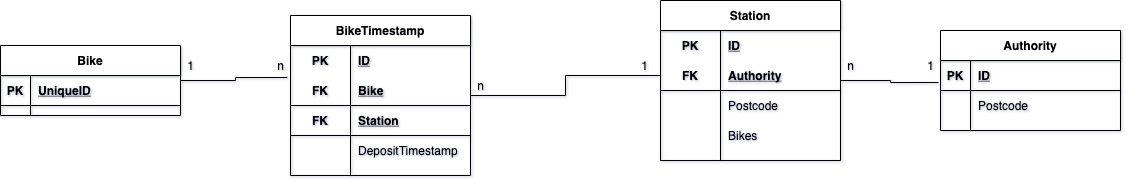
\includegraphics[width=\columnwidth]{bikesdw.png}
	\label{fig:bikesdw}
\end{figure}
\begin{enumerate}
	\item In Figure ~\ref{fig:bikes} each station counts the number of bikes
		deposited (summing one bike when it arrives to a certain counter, and
		subtracting the number when the bike leaves). The station stores the
		weekly data (such as the transactions), and sends the current sum to a
		central authority when it wants to know the sum of bikes in a specific
		time. 
		The station has an unique identifier, the postcode and the sum of the
		current parked bikes. Each station has a query interface that queries
		the number of bikes. The central authority has the postcode and name of the
		city, and a query interface to the stations to get the results of queries (3.a) and (3.b).
	\item Each bike has a RFID tag that identifies the vehicle and tells the
		station when it is parked. The DBMS of the sensor network is MadWise,
		because, as it provides timing mechanisms for queries (such as the
		support of the EVERY clause), and the stream-based data model, which
		makes manipulating the data easier. The central authority makes spatial
		queries to the devices to do further data analysis, and uses stream
		processing from Apache Spark to provide views of data of the various
		stations.
		\begin{verbatim}
			SELECT postcode, AVG(bikes)
			FROM station
			WHERE postcode = "00560" AND s.time = (CURRENT_TIMESTAMP - INTERVAL 1
			HOUR);
		\end{verbatim}
	\item 
		\begin{verbatim}
			SELECT postcode, COUNT(bikes)
			FROM station 
			WHERE postcode LIKE "0056[0-9]"
			EPOCH 15 minutes;
		\end{verbatim}
	\item It can be done by using the station to map the bikes and using an
		authority to reduce the stations. In detail, each station maps the postcode with the number 
		of bikes. The sum of
		all the station $(postcode, bikes) $ is reduced to a summation of each
		station, to provide the total number of bikes. 
		\begin{enumerate}
			\item Assuming that each station has run the query in (a) and sent
				the result to the central authority, 
				\begin{verbatim}
				SELECT AVG(bikes) 
				FROM stations
				WHERE postcode = "00560" AND time = (CURRENT_TIMESTAMP - INTERVAL 1 HOUR);			    
				\end{verbatim}
			\item What said above applies for (b)
				\begin{verbatim}
					SELECT SUM(bikes)
					FROM stations
					WHERE postcode LIKE "0056[0-9]" AND time =
					(CURRENT_TIMESTAMP - INTERVAL 15 MINUTES)
				\end{verbatim}
		\end{enumerate}
	\item 
		\begin{description}
			\item[Volume] The platform should be able to support huge amount of
				data coming from all the stations, as those can be many and
				dislocated in different areas of the city. 
			\item[Veracity] The data recorded by the stations should indicate
				the correct number of bikes parked. Otherwise, the system would
				be unreliable for the users.
			\item[Value] The data can be reused to benefit the users of the bike
				sharing system, such as telling how many bikes are available in
				a certain station. This can make possible to create a platform
				where a user can check if a bike is available, and reach a
				station to ride it. 
		\end{description}
	\item In Figure ~\ref{fig:bikesdw} there is a possible model of the
		database. Between the two implementations, it can be chosen to add
		redundant data to the table, to reduce the computations. The data
		representation language would be SQL, which is conceptualized in a
		UML schema.
	\item This can be done trough asymmetric key cryptography, where the
		sender (the station) can combine a short digital signature to the
		message using its private key. When the authority receives the message,
		it can use sender's public key to verify the the signature. If the
		signature matches the message, the origin is verified.
\end{enumerate}

% section data_management (end)
\section{Bonus 1} % (fold)
\label{sec:bonus_1}
\subsection{Introduction} % (fold)
\label{sub:containers}
Container technologies solve the problem of
virtualizing applications without by reducing the overhead of high level virtual 
machines, that "due to its inherent
ability for portability and extensibility [\ldots] it also enables
automated deployment, scaling and management of containerized applications \cite{8825476}.
Thanks to the increasing power in IoT devices, computational tasks are being shifted
to edge devices, but this increases the mantainability costs, and a scalable way
is needed. 
We have seen containerization in a master–slave architecture
where the communication between the master and slaves is
done using a kubelet device, which is a program that runs on each node and
communicates with the Kubernet server.
In the present, we want to analyze a possible use of containerization in a P2P
network, re-adapting the use-cases of \cite{8825476} and \cite{Mo2017} to a
Vehicular Ad-hoc NETwork (VANET). In the implementation of \cite{9102237} the
nodes of the network create a distribute file system, and communicate with a
distributed ledger are organized in a P2P architecture. The implementation
doesn't specifies the hardware and software configuration, hence there is the
possibility that containers could support the infrastructure. 
% subsection containers (end)

\subsection{Advantages} % (fold)
\label{sub:advantages}
Containerization can have positive advantages in a VANET, ranging from ease of
configuration, security, and performance.
Container technology can make easier to deploy a new smart device. Supposing that
we use Docker as a container system, 
let's have a new device that wants to join the ledger network. We can write a configuration 
file and run the container inside a
edge, automatically becomes a node of the network of vehicles. Containers represent an
 advantage over traditional virtual
machines, as they provide OS-level virtualization, which is faster than a
high level virtualization. Containers are simple to
configure (Docker uses a config files), and easy to replicate. As new vehicles are
manufactured and are purchased everyday, the manufacturer could download the
docker image, and run the system on the vehicle.\\
Additionally, we have observed several differences on the OS type of on board
 computers of different manufacturers. OS may be based on a different Linux
 distro, and maintainers of those systems need to update and compile the
 programs for each operating system. In contrast, containers don't need specific
 software dependency to be installed or to be compatible with the OS, since these are installed
inside the Linux-based container, and run inside the virtual machine.
This open ulterior security advantages, since a container isolates the running 
program from the host system. If the VANET is object of an attack, the attacker
cannot access the hardware resources. However,
introducing containerization creates an ulterior layer of attack, as bot the host
operating system and the container system can be attacked. Therefore it is
important to evaluate the possible risks in a containerized architecture.
% subsection advantages (end)

\subsection{Conclusion} % (fold)
\label{sub:conclusion}
In the light of this, containerization can be advantageous for P2P VANETs, as it
simplifies the configuration overhead, and provides a scalable architecture.
However, it is important to be aware of the limitations of containers, and the
possible vulnerabilities.

% subsection conclusion (end)

% section bonus_1 (end)

\bibliographystyle{ACM-Reference-Format}
\bibliography{references}

\end{document}

\endinput
%%
%% End of file `sample-acmsmall.tex'.

